\documentclass{standalone}

\usepackage{tikz}
    
\usepackage{graphicx} % Работа с графикой \includegraphics{}
\graphicspath{{./images/img1/}} % картинки в папке ./images/img1/
    
\begin{document}

\begin{tikzpicture}
    %\draw[help lines] (-6,-3) grid (10,3);
    \node at (-0.5,0)
        {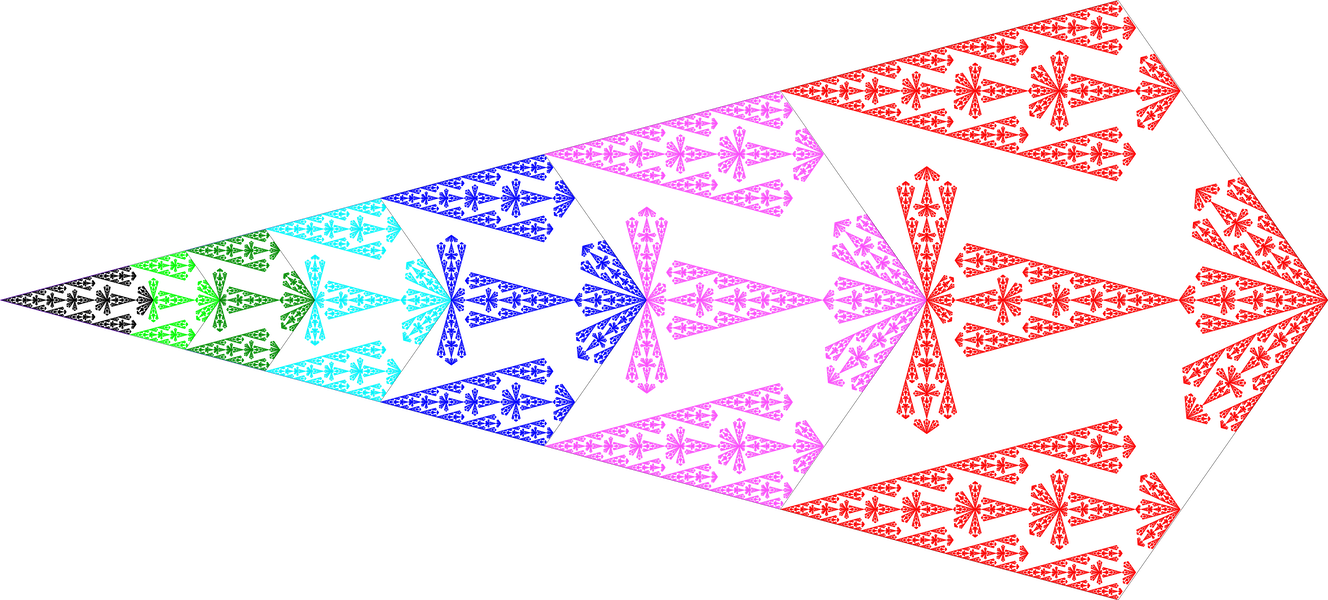
\includegraphics[width=11.05cm]{wdecomp.png}};
    \node at (8.5,-0.1)
        {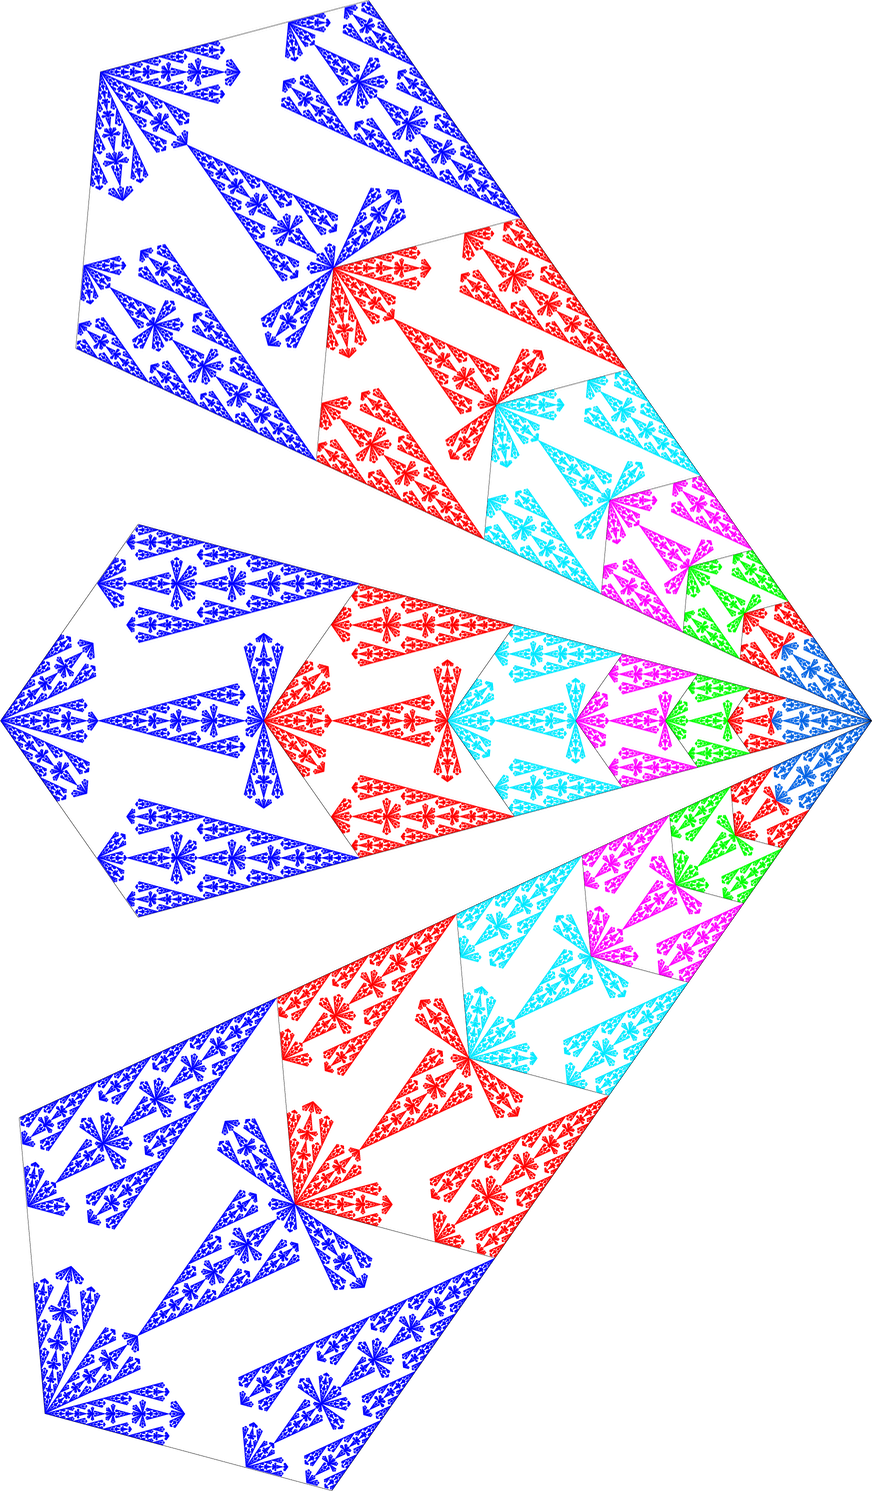
\includegraphics[width=3.06cm]{omdpwp.png}};
    \node at (1.5,2.5){$W$};
    \node at (-0.5,2){$S_1(W)$};
    \node at (-2.1,1.5){$S_1^2(W)$};
    \node at (-3.5,1){$S_1^3(W)$};
    \node at (-6,0.5){$B$};
    \node at(5.3,0){$A$};
    \node at(10.3,0){$A$};
    \node at(1.4,0){$C$};
    \draw[fill=black] 
        (-6,0)circle(0.06) 
        (1.7,0)circle(0.06) 
        (5,0)circle(0.06) 
        (10,0)circle(0.06);
\end{tikzpicture}

\end{document}